% Day 5 notes, SC Quantathon v3 Bootcamp. Build: latexmk -pdf notes.tex
\documentclass[11pt]{article}

\usepackage[margin=1in]{geometry}
\usepackage{lmodern}
\usepackage[T1]{fontenc}
\usepackage{microtype}
\usepackage{amsmath,amssymb}
\setlength{\arraycolsep}{3pt}
\usepackage{braket}
\usepackage{graphicx}
\usepackage{booktabs}
\usepackage{caption}
\usepackage{listings}
\usepackage{xcolor}
\usepackage[hidelinks]{hyperref}

\captionsetup{font=small,labelfont=bf}
\graphicspath{{figures/}}

\lstset{
  language=Python,
  basicstyle=\ttfamily\small,
  keywordstyle=\color{blue!60!black},
  commentstyle=\color{gray},
  stringstyle=\color{green!40!black},
  showstringspaces=false,
  frame=single,
  framerule=0.3pt,
  rulecolor=\color{gray!50},
  xleftmargin=1em,
  aboveskip=0.6em,
  belowskip=0.6em,
}

\newcommand{\code}[1]{\texttt{#1}}

\title{Day 5: Real Hardware: Transpilation, Noise, and Error Mitigation}
\author{SC Quantathon v3 Bootcamp \\ Clemson Quantum Club}
\date{}

\begin{document}
\maketitle

\noindent
Every earlier day ended with an optional cell that sent a circuit to a real processor and came back with a histogram slightly different from the simulator's. Today that difference is the subject. These notes follow the Day~5 notebook section by section: what a real machine is, how a circuit is rewritten to run on it, where each kind of error comes from, and two ways to get some of the lost accuracy back. Everything runs against \code{FakeSherbrooke}, a snapshot of \code{ibm\_sherbrooke}, a 127-qubit Eagle processor retired in July 2025, that carries its real calibration data and runs offline; the live machines today are Heron and Nighthawk processors, and everything the snapshot teaches carries over.

\section{Meet the machine}

A superconducting processor is a chip of transmon qubits held near 15~mK and driven by microwave pulses. Three facts about it decide what a circuit can do, and all three are attached to the backend object.

\begin{itemize}
\item The \emph{coupling map}: which pairs of qubits are physically connected. Sherbrooke has 127 qubits joined by 144 couplers in a heavy-hexagon lattice; no qubit touches more than three neighbours, and most touch two. The sparse lattice is a deliberate trade: fewer neighbours means fewer frequency collisions and less crosstalk between qubits that are driven at the same time, at the price of longer routes for circuits that want to connect distant qubits.
\item The \emph{native gates}: the operations the electronics can play. On Sherbrooke they are $R_z$, $\sqrt X$ (\code{sx}), $X$, and one two-qubit gate, the echoed cross-resonance gate \code{ecr}, which is a CNOT up to single-qubit corrections.
\item The \emph{calibration data}: how good each qubit and each gate currently is, remeasured every few hours.
\end{itemize}

Each qubit has a $T_1$, the time for an excited $\ket{1}$ to decay to $\ket{0}$; a $T_2$, the time for a superposition to lose its phase; and a \emph{readout error}, the chance that a measurement reports the wrong bit. Each coupler has a gate error and a duration. Table~\ref{tab:cal} gives the snapshot's medians, and Figure~\ref{fig:cal} the spread across the chip.

\begin{table}[h]
\centering
\small
\begin{tabular}{@{}lll@{}}
\toprule
quantity & median & notes \\
\midrule
$T_1$ & 278 $\mu$s & qubit 0: 382 $\mu$s \\
$T_2$ & 170 $\mu$s & qubit 0: 132 $\mu$s \\
readout error & 1.98\% & one qubit at 50\%, effectively dead \\
\code{ecr} gate error & 0.78\% & best pair (61, 60) at 0.35\%; nine pairs at 100\% \\
\code{ecr} duration & 533 ns & single-qubit gates are tens of ns \\
\bottomrule
\end{tabular}
\caption{Calibration data of the \code{ibm\_sherbrooke} snapshot.}
\label{tab:cal}
\end{table}

\begin{figure}[h]
\centering
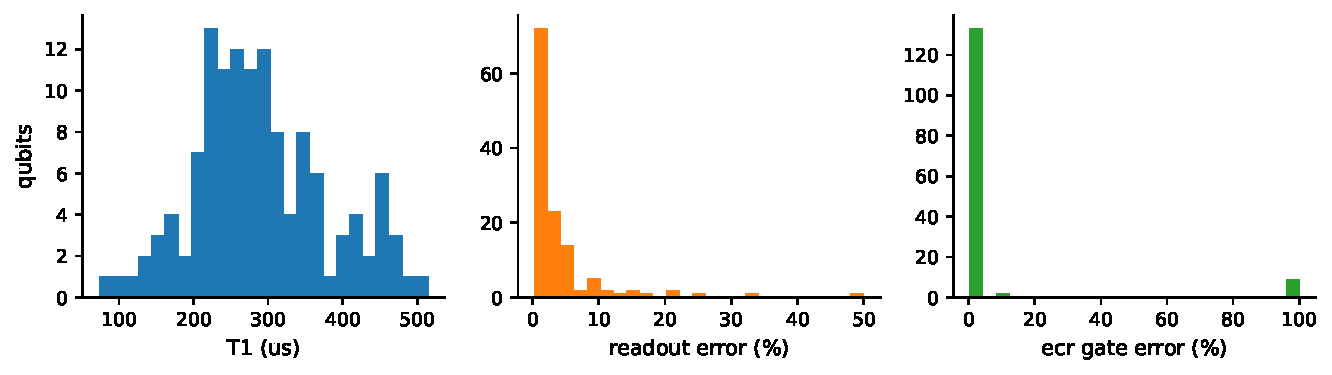
\includegraphics[width=0.98\textwidth]{calibration}
\caption{Calibration data across the 127 qubits and 144 couplers of the snapshot: $T_1$, readout error, and \code{ecr} gate error.}
\label{fig:cal}
\end{figure}

Two lessons hide in the table. Calibration data are measurements, not specifications: a few qubits report $T_2 > 2T_1$, which physics forbids, and a few qubits and couplers report errors of 50\% or 100\%, which means ``currently unusable'' rather than a number to plug in. And the time scales are separated by two orders of magnitude: a two-qubit gate takes half a microsecond against coherence times of hundreds of microseconds, so a circuit of depth twenty runs in about ten microseconds and loses only a few percent to decoherence. For short circuits the two-qubit gate error, at roughly a percent per gate, matters first.

\section{Transpilation}

The circuits you write use $H$, CNOT, and whatever else is convenient, on qubits numbered from zero. The chip runs only its native gates, only between coupled pairs, on physical qubits of its choosing. The \emph{transpiler} bridges the gap with three jobs, which Qiskit runs as layout, routing, translation, and then an optimization pass:
\begin{enumerate}
\item choose a \emph{layout} of the circuit's qubits onto physical qubits, preferring good ones;
\item \emph{route}, inserting SWAP gates wherever a two-qubit gate needs a pair that is not coupled, each SWAP costing three two-qubit gates;
\item \emph{translate} every gate into native ones, using identities such as $H = R_z(\tfrac\pi2)\sqrt X R_z(\tfrac\pi2)$ up to phase.
\end{enumerate}
The result is an \emph{ISA circuit} (instruction set architecture), the only kind a real backend accepts. The Bell circuit's one $H$ and one CNOT become seven $R_z$, four $\sqrt X$, and one \code{ecr}, and the depth grows from 3 to 8; the two logical qubits land on physical qubits 0 and 1.

A few circuit tools help in reading the result. A \emph{barrier} is a visual divider that also stops the optimizer from merging gates across it. \code{measure(q, c)} stores one qubit into one bit of a classical register you declared; \code{measure\_all()} adds a register named \code{meas} and measures every qubit. \code{depth()} counts the layers of gates that cannot run at the same time, and \code{count\_ops()} counts gates by name. Figure~\ref{fig:native} shows the translation step alone on the one-qubit circuit $H, T, H$: three gates become five, of the kinds $R_z$ and $\sqrt X$ only, and \code{Operator.equiv} confirms the two circuits are the same unitary up to a global phase. The notebook's version of the same cell keeps a barrier between $T$ and the second $H$, which stops the translator from merging two adjacent $R_z$ gates, so it reports four $R_z$ instead of three: a barrier costs nothing on the chip but can cost an optimization.

\begin{figure}[h]
\centering
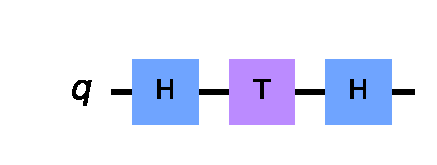
\includegraphics[width=0.28\textwidth]{hth_circuit}\hfill
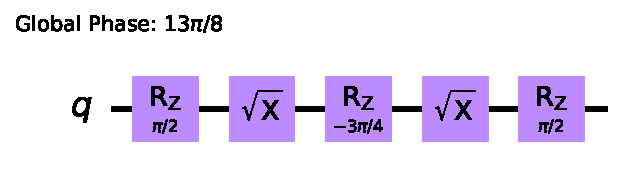
\includegraphics[width=0.62\textwidth]{hth_native}
\caption{The circuit $H, T, H$ as written (left, depth 3) and translated to IBM's native gate set (right, depth 5: three $R_z$ and two $\sqrt X$).}
\label{fig:native}
\end{figure}

The \emph{optimization level}, 0 to 3, controls how hard the transpiler works to shorten the result by cancelling adjacent gates, merging rotations, and searching for a better layout. Table~\ref{tab:levels} shows a five-qubit GHZ circuit at each level. Level 0 does the minimum; level 1 is the fastest and, for this circuit, also the shortest, because the linear chain of CNOTs already fits the lattice; levels 2 and 3 choose a different layout and land on a slightly longer circuit, so a higher level is not guaranteed to be shorter. The number of two-qubit gates is the figure to watch, since those carry most of the error.

\begin{table}[h]
\centering
\small
\begin{tabular}{@{}llll@{}}
\toprule
optimization level & depth & \code{ecr} gates & all gates \\
\midrule
0 & 32 & 4 & 71 \\
1 & 17 & 4 & 37 \\
2 & 25 & 4 & 48 \\
3 & 25 & 4 & 48 \\
\bottomrule
\end{tabular}
\caption{A five-qubit GHZ circuit (1 $H$, 4 CNOTs) transpiled for the snapshot at each optimization level.}
\label{tab:levels}
\end{table}

Routing shows its cost on a machine whose lattice does not match the circuit. \code{FakeManilaV2} is five qubits in a line, 0--1--2--3--4. A star circuit with CNOTs from qubit 0 to each of the others cannot run directly, because qubit 0 touches only qubit 1. At level 3 the transpiler produces 10 native CNOTs for the 4 logical ones and a depth of 14: the extra six are two SWAPs. On a real job, routing overhead of this kind is often the single largest source of error, which is why the layout step tries so hard to avoid it. The arithmetic is unforgiving: a SWAP is three CNOTs (Day~4), so at a percent of error per two-qubit gate each routed SWAP costs about three percent of fidelity, and a circuit that needs ten of them has lost a quarter of its signal before any of its own gates have run. Layout is therefore a search: the transpiler tries to find a placement of the logical qubits on the coupling map under which every two-qubit gate already sits on a coupler, and only when no such placement exists does it route.

\section{Where errors come from}

Three mechanisms account for nearly everything that separates a real run from the simulator. Each has a simple model, and \code{qiskit\_aer.noise} can attach any of them to a circuit, so each can be studied alone before they are mixed.

\subsection{Decoherence}

An excited qubit relaxes to its ground state at a constant rate, so after an idle time $t$ the state $\ket{1}$ has survived with probability
\begin{equation}
P(1) = e^{-t/T_1} .
\label{eq:t1}
\end{equation}
A superposition also loses its phase. The relative phase of $\ket{+}$ drifts randomly, and averaging over the drift shrinks the $x$ component of the Bloch vector by $e^{-t/T_2}$, so a measurement in the $X$ basis returns $+$ with probability
\begin{equation}
P(+) = \tfrac12\big(1 + e^{-t/T_2}\big) ,
\label{eq:t2}
\end{equation}
which decays from 1 toward $\tfrac12$: a fully dephased qubit is a fair coin in every basis. Both curves come from the same assumption, a constant rate: if an excited qubit decays with probability $dt/T_1$ in every short interval $dt$, then $dP/dt = -P/T_1$ and $P(t) = e^{-t/T_1}$, the same law as radioactive decay. Relaxation also destroys phase, and it does so at half the rate: the off-diagonal element of the density matrix that carries the coherence decays as $e^{-t/2T_1}$ from relaxation alone, so $1/T_2 = 1/(2T_1) + 1/T_\varphi$ with $T_\varphi$ the pure dephasing time, and $T_2 \le 2T_1$ with equality only when nothing but relaxation is happening. Figure~\ref{fig:decoherence} is both curves for qubit 0 of the snapshot, produced by the \code{thermal\_relaxation\_error} channel with that qubit's $T_1$ and $T_2$.

\begin{figure}[h]
\centering
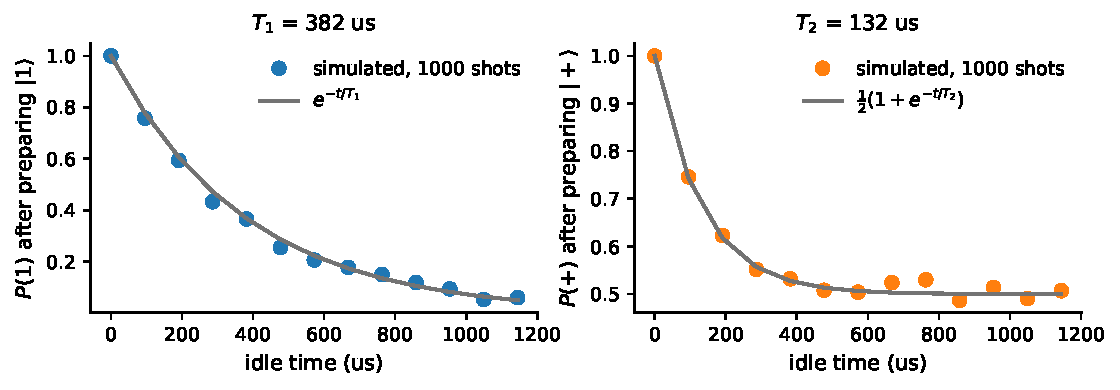
\includegraphics[width=0.98\textwidth]{decoherence}
\caption{Decoherence of qubit 0 of the snapshot, simulated with its calibrated $T_1 = 382\ \mu$s and $T_2 = 132\ \mu$s. Left: survival of $\ket{1}$, Eq.~\eqref{eq:t1}. Right: survival of the phase of $\ket{+}$, Eq.~\eqref{eq:t2}.}
\label{fig:decoherence}
\end{figure}

\subsection{Gate error}

Each gate is a pulse that is slightly wrong. The simplest model is \emph{depolarizing} noise: after each gate, with probability $p$ the state is replaced by the maximally mixed state, which is equally likely to be anything. After $k$ gates the chance that no scrambling has occurred is $(1-p)^k$, and a scrambled two-qubit state still reads \code{00} a quarter of the time, so a chain of $k$ CNOTs, which is the identity on paper when $k$ is even, returns \code{00} with probability
\begin{equation}
P(00) = \tfrac14 + \tfrac34\,(1 - p)^k .
\label{eq:depol}
\end{equation}
Where the quarter comes from: the depolarizing channel maps the two-qubit density matrix to $\rho \mapsto (1-p)\rho + p\,I/4$, and applying it $k$ times gives $\rho_k = (1-p)^k\rho + \big(1 - (1-p)^k\big)I/4$, since the maximally mixed state is a fixed point. Reading off $\braket{00|\rho_k|00}$ with $\rho = \ket{00}\bra{00}$ gives $(1-p)^k + \tfrac14(1 - (1-p)^k)$, which is Eq.~\eqref{eq:depol}. Figure~\ref{fig:cnot} tests it at $p = 1\%$: the formula predicts $0.863$ and $0.752$ at $k = 20$ and $40$, and the simulation measures 0.866 and 0.754. This is a gate-repetition experiment. The standard hardware method, \emph{randomized benchmarking}, applies sequences of random Clifford gates followed by an inverting gate, which averages coherent errors into exactly this depolarizing decay.

\begin{figure}[h]
\centering
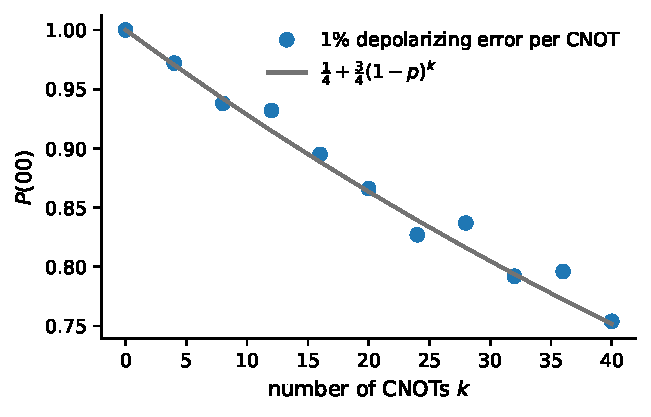
\includegraphics[width=0.55\textwidth]{cnot_decay}
\caption{$P(00)$ after $k$ CNOTs with 1\% depolarizing error per gate, and Eq.~\eqref{eq:depol}.}
\label{fig:cnot}
\end{figure}

\subsection{Readout error}

The last step has its own error: a $\ket{0}$ is sometimes reported as 1 and a $\ket{1}$ as 0, at rates that differ. The two rates make a $2\times2$ \emph{confusion matrix} whose columns are the prepared state and whose rows are the reported one. For one qubit the matrix is
\begin{equation}
M = \begin{pmatrix}1 - \epsilon_0 & \epsilon_1\\ \epsilon_0 & 1 - \epsilon_1\end{pmatrix},
\label{eq:confusion}
\end{equation}
with $\epsilon_0$ the chance of reading 1 when $\ket{0}$ was prepared and $\epsilon_1$ the reverse; on the snapshot the two are typically a percent or two each and unequal, since a $\ket{1}$ can also decay during the readout pulse. When the qubits read out independently, the two-qubit matrix is the tensor product $M_1\otimes M_0$ of the single-qubit ones. For a 50/50 state a symmetric error ($\epsilon_0 = \epsilon_1$) moves as many counts one way as the other and changes nothing, which is why Day~1's random-bit histogram showed no sign of it; only the asymmetry shifts the counts. Readout error is the easiest to correct, because it acts after the circuit and its matrix can be measured directly.

\section{Simulating the machine}

\code{AerSimulator.from\_backend} assembles all three mechanisms from the calibration data, thermal relaxation on every gate, depolarizing error at the measured rates, and each qubit's readout error, and runs an ISA circuit through them. It is the best offline prediction of what the machine will do. The prediction has limits worth knowing: the model treats every error as independent and memoryless, so it misses crosstalk between simultaneous gates, coherent errors that add up in phase rather than at random, and drift between the calibration and the run, which together explain why a real device is usually somewhat worse than its snapshot. Table~\ref{tab:three} and Figure~\ref{fig:three} compare the ideal simulator, the noisy simulator, and Day~4's recorded run of the same Bell circuit on \code{ibm\_kingston}, a Heron r2 processor whose two-qubit gate is \code{cz}, on physical qubits 55 and 59. The noisy simulator predicts 3.0\% impossible outcomes and the device showed 1.0\%; the Hellinger fidelities to the ideal histogram are 0.970 and 0.990. The two agree on the scale of the error, a percent or so, and not on the number, and the direction is the informative part: the snapshot is of an Eagle machine retired in 2025, while the live run used a current processor on a pair chosen from that day's calibration table, so the device did better than the old snapshot predicts. A snapshot of the same machine on the same day would be expected to land closer.

\begin{table}[h]
\centering
\small
\begin{tabular}{@{}lllll@{}}
\toprule
& counts (\code{00}, \code{01}, \code{10}, \code{11}) & impossible outcomes & fidelity to ideal \\
\midrule
ideal simulator & 506, 0, 0, 494 & 0\% & 1.000 \\
noisy simulator & 504, 13, 17, 466 & 3.0\% & 0.970 \\
\code{ibm\_kingston}, Day~4 run & 512, 6, 4, 478 & 1.0\% & 0.990 \\
\bottomrule
\end{tabular}
\caption{The Bell circuit three ways.}
\label{tab:three}
\end{table}

\begin{figure}[h]
\centering
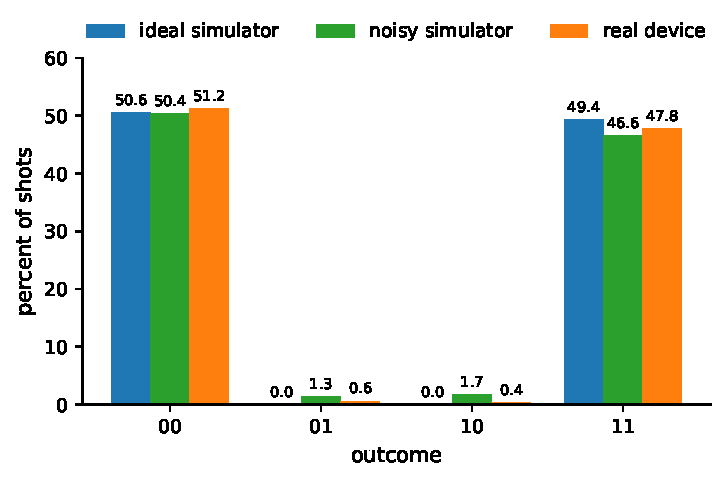
\includegraphics[width=0.62\textwidth]{bell_three_ways}
\caption{The Bell circuit on the ideal simulator, on the noisy simulation of the snapshot, and on \code{ibm\_kingston} (Day~4's run).}
\label{fig:three}
\end{figure}

\section{Readout error mitigation}

Readout error acts after the circuit, so linear algebra can undo it. Prepare each basis state in turn on the same physical qubits the circuit uses, measure it, and record the distribution of reported strings. That fills a matrix $M$ whose entry $M_{ij}$ is the probability of reading $i$ when $j$ was prepared. A measured distribution is then $\vec p_{\rm meas} = M\vec p_{\rm true}$, and
\begin{equation}
\vec p_{\rm true} = M^{-1}\vec p_{\rm meas}
\label{eq:mitigate}
\end{equation}
recovers the distribution the circuit would have produced with perfect readout. For two qubits $M$ is $4\times4$ and needs four calibration circuits. Statistical noise can push entries of the solution slightly negative; clipping and renormalizing is the standard fix.

For the Bell circuit on physical qubits 0 and 1 of the snapshot, the measured $M$ has diagonal entries 0.964, 0.965, 0.966, 0.965, and applying Eq.~\eqref{eq:mitigate} to the noisy counts drops the impossible outcomes from 3.0\% to 0.0\% (Figure~\ref{fig:readout}). Inversion has a price. $M^{-1}$ has entries slightly larger than one on the diagonal and small negative entries off it, so it amplifies the statistical noise of the counts by a few percent for a matrix like this one, and by much more when readout is poor and $M$ is far from the identity. It also scales badly: a full $M$ for $n$ qubits is $2^n\times2^n$ and needs $2^n$ calibration circuits, so beyond a handful of qubits the per-qubit form of Eq.~\eqref{eq:confusion} is measured instead and the tensor product is assumed. What survives mitigation is the error that happened \emph{inside} the circuit, mostly the two-qubit gate, which this method cannot touch. On the runtime, \code{EstimatorV2} with \code{resilience\_level = 1} performs this calibration automatically, using a technique called TREX.

\begin{figure}[h]
\centering
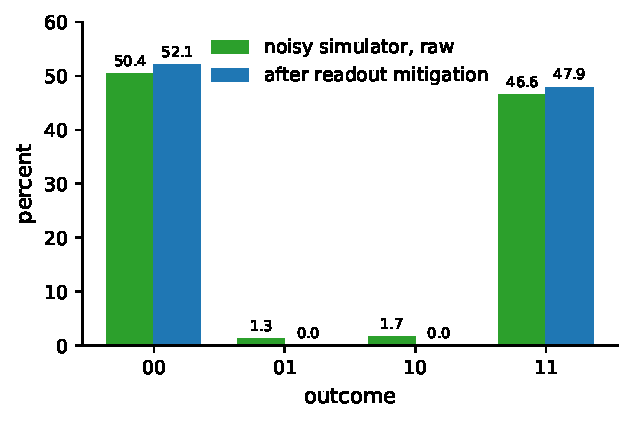
\includegraphics[width=0.55\textwidth]{readout_mitigation}
\caption{The noisy simulator's Bell counts before and after readout error mitigation with a measured confusion matrix.}
\label{fig:readout}
\end{figure}

\section{Zero-noise extrapolation}

Gate error cannot be calibrated away, but it can be amplified on purpose and extrapolated out. Replace every CNOT by three CNOTs, the same gate on paper and three times the gate error in practice, then by five. An expectation value measured at noise scales $\lambda = 1, 3, 5$ traces a curve, and the value of that curve at $\lambda = 0$ estimates the noiseless result. This is \emph{zero-noise extrapolation} (ZNE). For $\braket{ZZ}$ of the Bell state, exactly 1 without noise, a CNOT with 3\% depolarizing error gives $0.9677$, $0.9100$, and $0.8603$ at the three scales (Figure~\ref{fig:zne}). The simplest version uses two points: if the error is linear in $\lambda$, then $E(\lambda) = E_0 + a\lambda$, and the measurements at $\lambda = 1$ and $3$ give $E_0 = (3E_1 - E_3)/2$, which here is $(3\times0.9677 - 0.9100)/2 = 0.997$. A straight line fitted through all three points reaches $0.9932$ at $\lambda = 0$ and a quadratic reaches $0.9995$, against the unmitigated $0.9677$. Folding works because a CNOT is its own inverse, so $\mathrm{CNOT}^3 = \mathrm{CNOT}$ exactly on paper; for a general gate $G$ the fold is $G\,G^\dagger G$, the same identity. Both recover most of the lost $0.03$; the quadratic lands within a thousandth of the true value because the exact decay, $(1-p)^{\lambda}$ up to the $\tfrac14$ offset, is curved, and a fit that can bend follows it better. An extrapolation inherits the scatter of its inputs, so with fewer shots either fit can also overshoot 1.

\begin{figure}[h]
\centering
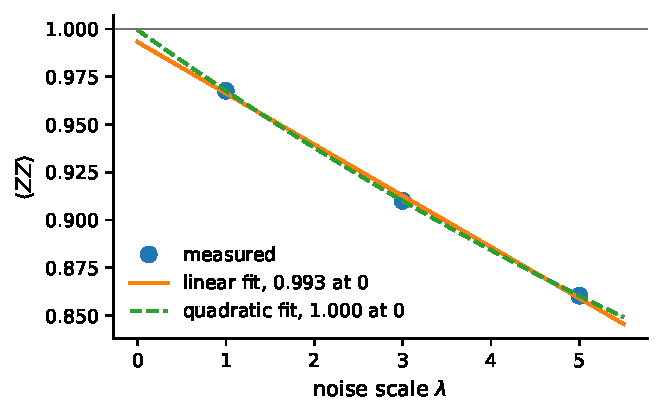
\includegraphics[width=0.55\textwidth]{zne}
\caption{Zero-noise extrapolation of $\braket{ZZ}$ for the Bell state under 3\% depolarizing CNOT error. The three points are measured at noise scales 1, 3, and 5; the fits are read off at scale 0.}
\label{fig:zne}
\end{figure}

ZNE costs three runs instead of one and returns an extrapolation, not a measurement, so its error bars are larger and it can overshoot. Its strength is that it needs no model of the noise. On the runtime, \code{EstimatorV2} with \code{options.resilience.zne\_mitigation = True} does the folding and fitting itself.

\section{The live machine}

Everything above used the snapshot. The notebook's last section sends the same Bell circuit to the least busy live processor, which was again \code{ibm\_kingston} on physical qubits 55 and 59, and this time it sends two jobs. The first is a Sampler job of five circuits: the Bell circuit and the four calibration circuits of Section~5, transpiled onto the same pair, so that the confusion matrix is measured on the qubits that actually ran rather than borrowed from the snapshot. The second is an Estimator job for $\braket{ZZ}$ with the runtime's own readout mitigation (TREX) and zero-noise extrapolation switched on, Sections~5 and 6 done by the service. Table~\ref{tab:live} and Figure~\ref{fig:live} hold the results.

\begin{table}[h]
\centering
\small
\begin{tabular}{@{}lll@{}}
\toprule
& value & note \\
\midrule
raw counts (\code{00}, \code{01}, \code{10}, \code{11}) & 527, 6, 4, 463 & 1.0\% impossible, fidelity 0.989 \\
confusion matrix diagonal on the pair & 0.999, 0.985, 0.995, 0.992 & readout error 0.1\% to 1.5\% \\
readout-mitigated probabilities & 0.527, 0.005, 0.001, 0.467 & \\
$\braket{ZZ}$, exact & 1.0000 & \\
$\braket{ZZ}$, snapshot ZNE (Section~6) & 0.9995 & quadratic fit \\
$\braket{ZZ}$, device raw & 0.9800 & from the raw counts \\
$\braket{ZZ}$, device readout mitigated & 0.9884 & with the on-device matrix \\
$\braket{ZZ}$, device with TREX and ZNE & 0.9952 & the runtime Estimator \\
\bottomrule
\end{tabular}
\caption{The Bell circuit on \code{ibm\_kingston}, physical qubits 55 and 59, 1000 shots per circuit.}
\label{tab:live}
\end{table}

\begin{figure}[h]
\centering
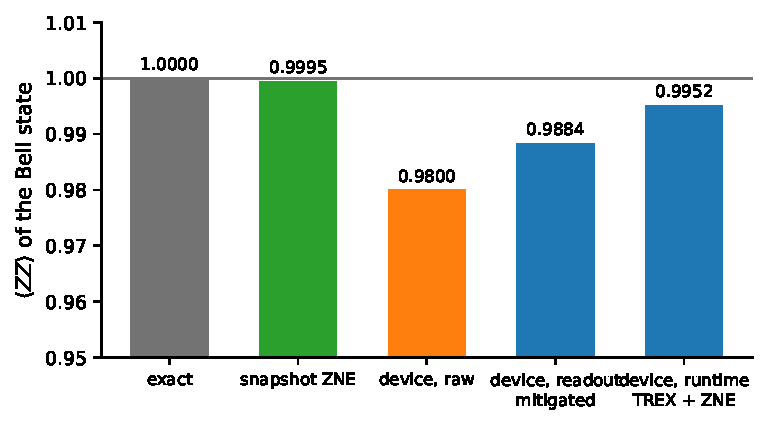
\includegraphics[width=0.66\textwidth]{live_zz}
\caption{$\braket{ZZ}$ of the Bell state, exact and as estimated five ways; the axis starts at 0.95.}
\label{fig:live}
\end{figure}

Two things are worth reading off. Readout mitigation barely moves this run, because the pair's readout is already at the percent level, so the ten impossible shots and the tilt between \code{00} and \code{11} (527 against 463, about two $\sigma$) came from inside the circuit: the \code{cz} gate and relaxation during it. That is exactly what the readout matrix cannot touch, and exactly what zero-noise extrapolation is for: the runtime's TREX plus ZNE takes $\braket{ZZ}$ from $0.980$ to $0.995$, three quarters of the way to the exact value, and it did so by running folded copies of the circuit and fitting, as Section~6 did on the snapshot. The remaining half percent is the price of extrapolating from noisy points. A second lesson is in the pair itself: the same two qubits gave 1.0\% impossible outcomes on Day~4 and 1.0\% here, an hour apart, while qubit~0 of the same chip was misreading half its zeros on Days~1 and 2. Which qubits a job lands on matters more than which machine.

\section{Summary}

\begin{itemize}
\item A backend carries a coupling map, a native gate set, and calibration data: $T_1$, $T_2$, and readout error per qubit; error and duration per coupler. Fake backends are offline snapshots with the same data, and a few qubits in any snapshot are effectively dead.
\item The transpiler lays out logical qubits onto physical ones, routes with SWAPs where the lattice requires, and translates gates to native ones. Two-qubit gate count is the cost that matters. Only ISA circuits run on hardware.
\item $\ket{1}$ survives as $e^{-t/T_1}$ and a superposition keeps its phase as $e^{-t/T_2}$, Eqs.~\eqref{eq:t1} and~\eqref{eq:t2}. Depolarizing gate error compounds as $(1-p)^k$, Eq.~\eqref{eq:depol}. Readout error is a confusion matrix applied after the circuit.
\item \code{AerSimulator.from\_backend} combines the three from calibration data; for the Bell state its impossible-outcome fraction lands within two percent of the device's, with the current processor beating the retired snapshot (Table~\ref{tab:three}).
\item Readout mitigation inverts the measured confusion matrix, Eq.~\eqref{eq:mitigate}. Zero-noise extrapolation folds gates to amplify noise and extrapolates to zero. The runtime Estimator offers both as options.
\item On the live machine the readout matrix measured on the pair removed little, because readout was already at the percent level; the runtime's TREX plus ZNE moved $\braket{ZZ}$ from $0.980$ to $0.995$ (Table~\ref{tab:live}).
\end{itemize}

\begin{thebibliography}{9}
\bibitem{transpile} IBM Quantum documentation, \emph{Introduction to transpilation}. \url{https://quantum.cloud.ibm.com/docs/en/guides/transpile}
\bibitem{mitigation} IBM Quantum documentation, \emph{Error mitigation and suppression techniques}. \url{https://quantum.cloud.ibm.com/docs/en/guides/error-mitigation-and-suppression-techniques}
\bibitem{noise} IBM Quantum documentation, \emph{Building noise models} with Qiskit Aer. \url{https://quantum.cloud.ibm.com/docs/en/guides/build-noise-models}
\bibitem{krantz} P.~Krantz, M.~Kjaergaard, F.~Yan, T.~P. Orlando, S.~Gustavsson, and W.~D. Oliver, ``A quantum engineer's guide to superconducting qubits,'' Applied Physics Reviews \textbf{6}, 021318 (2019).
\bibitem{temme} K.~Temme, S.~Bravyi, and J.~M. Gambetta, ``Error mitigation for short-depth quantum circuits,'' Phys. Rev. Lett. \textbf{119}, 180509 (2017).
\bibitem{nielsen} M.~A. Nielsen and I.~L. Chuang, \emph{Quantum Computation and Quantum Information}, 10th anniversary ed. (Cambridge University Press, 2010), chapter 8, for the channels behind Eqs.~\eqref{eq:t1} to~\eqref{eq:depol}.
\end{thebibliography}

\end{document}
